\chapter{Симуляция базовых эмоций в трёхмерной модели}
\label{chap:results}
В системе, полученной из трёх совмещённых систем нейромодуляторов на языке Python, с общим словарём областей мозга, выделенными для них нейронами в реалистичных пропорциях и настроенными связями, была проведена симуляция на 150 000 нейронов. Симулировалась работа мозга в течение 1400 миллисекунд, за это время нейромодуляторы принимали различные значения, приводящие мозг в 8 различных состояний:


1. Эмоция «тоска/горе». Требует высокого уровня норадреналина при низких уровнях дофамина и серотонина. Генераторы спайков подключены к ядрам солитарного тракта, ядрам paragigantocellular, латерально-спинному ядру покрышки и perirphinal cortex с 100 по 200 мс.


2. Эмоция «испуг/ужас». Формируется при высоком уровне дофамина и низких уровнях серотонина и норадреналина. Генераторы спайков подключены к моторной коре, чёрной субстанции pars compacta, миндалевидному телу и вентральной области покрышки с 300 по 400 мс.


3. Эмоция «злость/ярость». Возникает при высоких уровнях норадреналина и  дофамина, а активность одного из них всегда влечёт активность другого. С 500 по 600 мс генерируются спайки на ядрах солитарного тракта, ядрах paragigantocellular, латерально-спинном ядре покрышки и perirphinal cortex. Вместе с ними работают генераторы на моторной коре, чёрной субстанции pars compacta, миндалевидном теле и вентральной области покрышки.


4. Эмоция «презрение/отвращение». Требует высокого уровня серотонина при низких уровнях дофамина и норадреналина. Генераторы спайков с 700 по 800 мс подключены к серотониновым очагам в префронтальной коре, моторной коре и ядрах шва (дорсальном и среднем).


5. Эмоция «удивление». Высокие уровни серотонина и норадреналина, норадреналин борется за сохранение своего возбуждающего влияния, но не в полной мере сохраняет его под ингибирующим действием серотонина. К генераторам в префронтальной коре, моторной коре, дорсальном и среднем ядрах шва добавляются генераторы на ядрах солитарного тракта, ядрам paragigantocellular, латерально-спинному ядру покрышки и perirphinal cortex, вместе они работают с 900 по 1000 мс.


6. Эмоция «радость/удовольствие». Требует одновременного существования спайковой активности в центрах дофамина и серотонина, концентрация норадреналина должна оставаться низкой. С 1100 по 1200 мс подключены генераторы к префронтальной коре, моторной коре, ядрам шва, чёрной субстанции pars compacta, миндалевидному телу и вентральной области покрышки.


7. Эмоция «интерес/азарт». Высокие уровни всех трёх нейромедиаторов. Генераторы спайков в центрах дофамина (моторной коре, чёрной субстанции pars compacta, миндалевидном теле и вентральной области покрышки), генераторы в центрах серотонина (префронтальная кора, моторная кора, дорсальное и среднее ядра шва), генераторы активности норадреналина (на ядрах солитарного тракта, ядрах paragigantocellular, латерально-спинном ядре покрышки и perirphinal cortex) включаются одновременно на 1300 мс, работают до 1400 мс.


8. Эмоция «стыд/унижение». Пониженные уровни всех трёх нейромедиаторов в промежутках между остальными выражаемыми эмоциями.


На сервере CISCO симуляция, распределённая на 8 потоков, заняла 17 часов, поскольку была намеренно облегчена нагрузка: детекторы спайков и вольтметры были подключены лишь к наиболее важным для анализа областям мозга. Этими частями стали: \begin{itemize}
\item Нейромодулирующие центры (ядра шва, голубоватое пятно, чёрная субстанция pars compacta);
\item Интерфейсы нейромодуляторов (стриатум, таламус, вентральная область покрышки);
\item Главные области, испытывающие проекции всех нейромодуляторов (моторная кора, сенсорная кора, префронтальная кора).
\end{itemize}



\begin{figure}
	\centering
	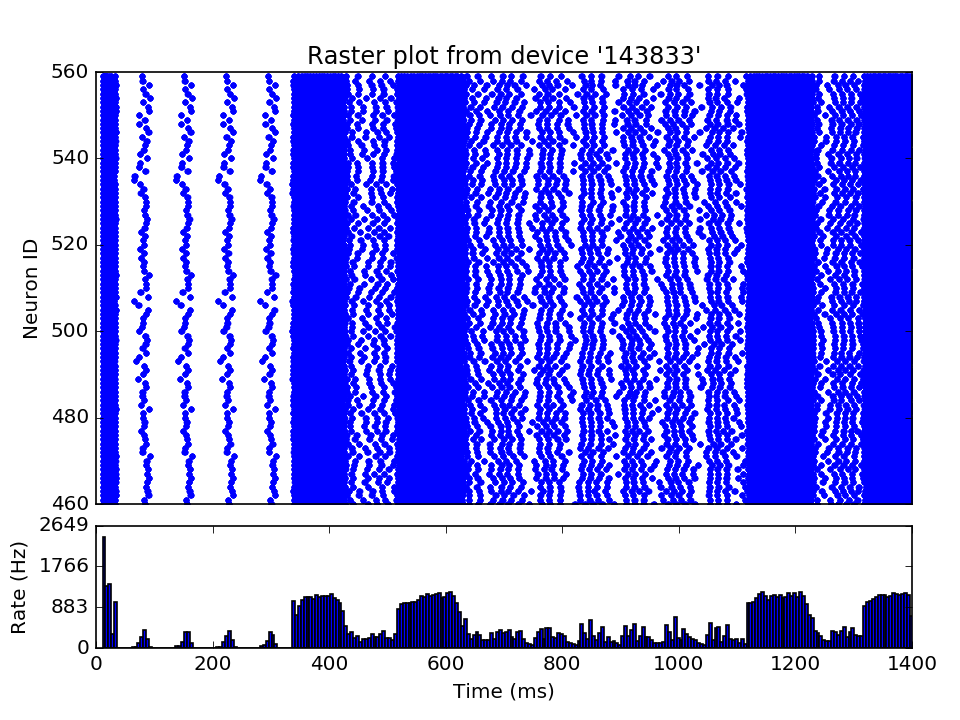
\includegraphics[width=0.5\linewidth]{spikes_lc[d1]}
	\caption{Спайковая активность в голубоватом ядре.}
	\label{fig:spikes_lc}
\end{figure}

\begin{figure}
	\centering
	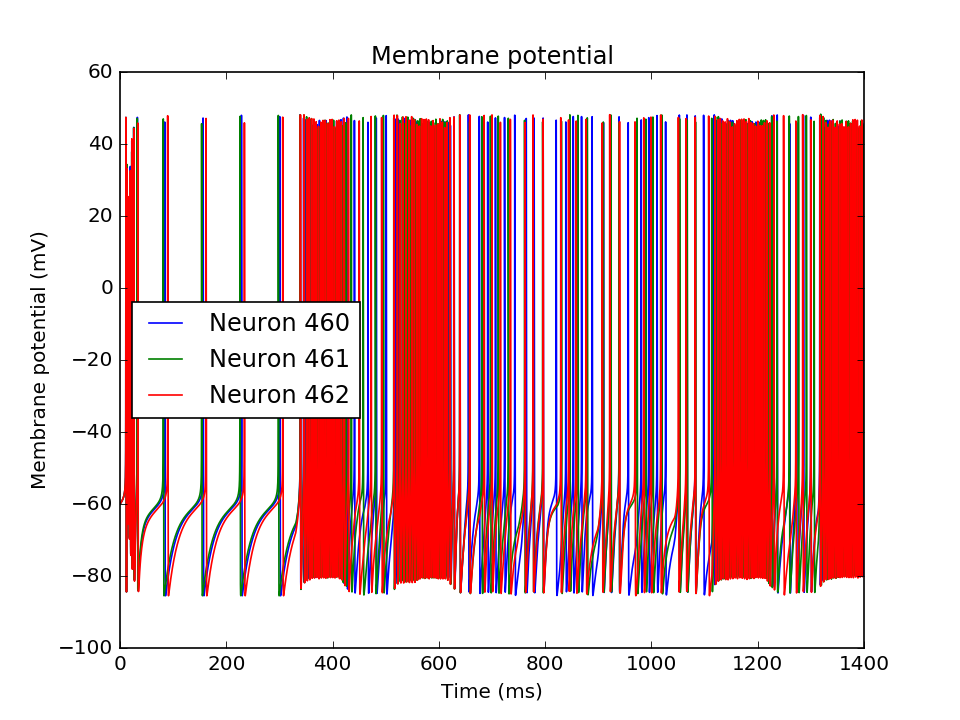
\includegraphics[width=0.5\linewidth]{volt_lc[d1]}
	\caption{Изменение потенциала мембраны нескольких нейронов в голубоватом ядре.}
	\label{fig:volt_lc}
\end{figure}

\begin{figure}
	\centering
	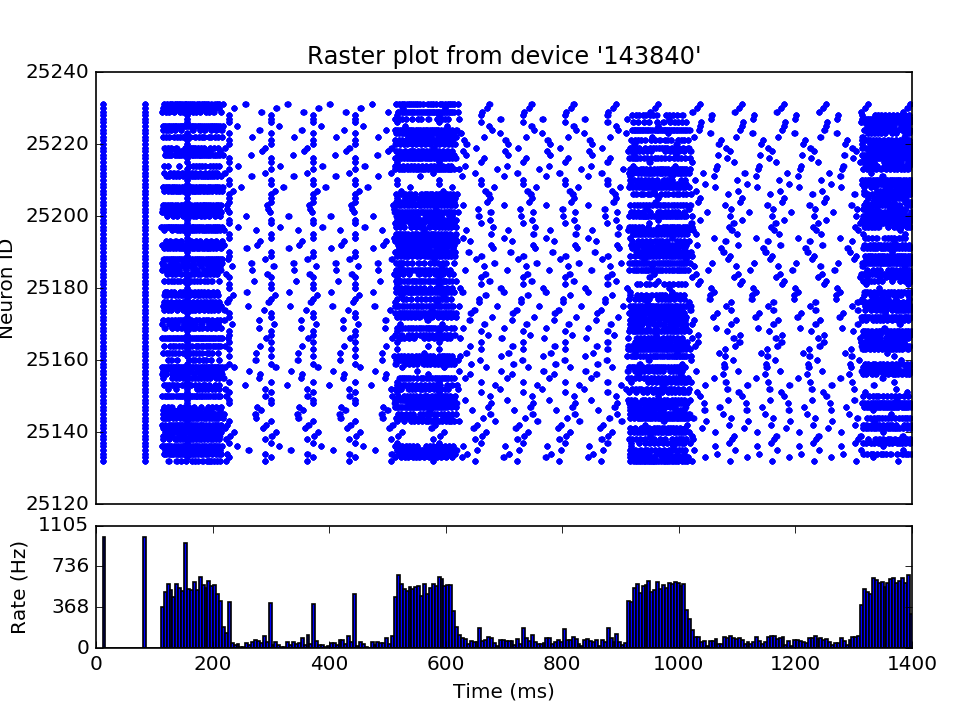
\includegraphics[width=0.5\linewidth]{spikes_nts[a1]}
	\caption{Спайковая активность в ядрах cолитарного тракта.}
	\label{fig:spikes_nts}
\end{figure}

На рис.  ~\ref{fig:spikes_lc} отображена спайковая активность в голубоватом ядре, главной области норадренергических нейронов. Активность заметно возрастает на 400 мс (испуг), 600 мс (ярость), 1200 мс (радость) и 1400 мс (интерес), именно в это время в системе была повышенная концентрация дофамина, который проецируется на голубоватое ядро, таким образом дополнительно активируя норадреналин. Увеличение частоты спайкования подтверждается на рис. ~\ref{fig:volt_lc}, где изменение потенциала мембраны трёх нейронов голубоватого пятна имеет форму классического спайка, который у показанных отдельных нейронов начинает происходить чаще в моменты подключения дофамина, в полном соответствии с рис.  ~\ref{fig:spikes_lc}. Ядра солитарного тракта --- второй центр норадреналина --- не показали такой же яркой зависимости от дофамина (рис. ~\ref{fig:spikes_nts}), активность в них усиливается на эмоциях, соответствующих норадреналину, за который ядра отвечают: 200 мс (горе), 600 мс (ярость), 1000 мс (удивление) и 1400 мс (интерес). Спайки, в меньшем количестве, присутствуют и в остальные моменты симуляции, что реалистично и объясняется проекциями из других областей на эту область мозга.

\begin{figure}
	\centering
	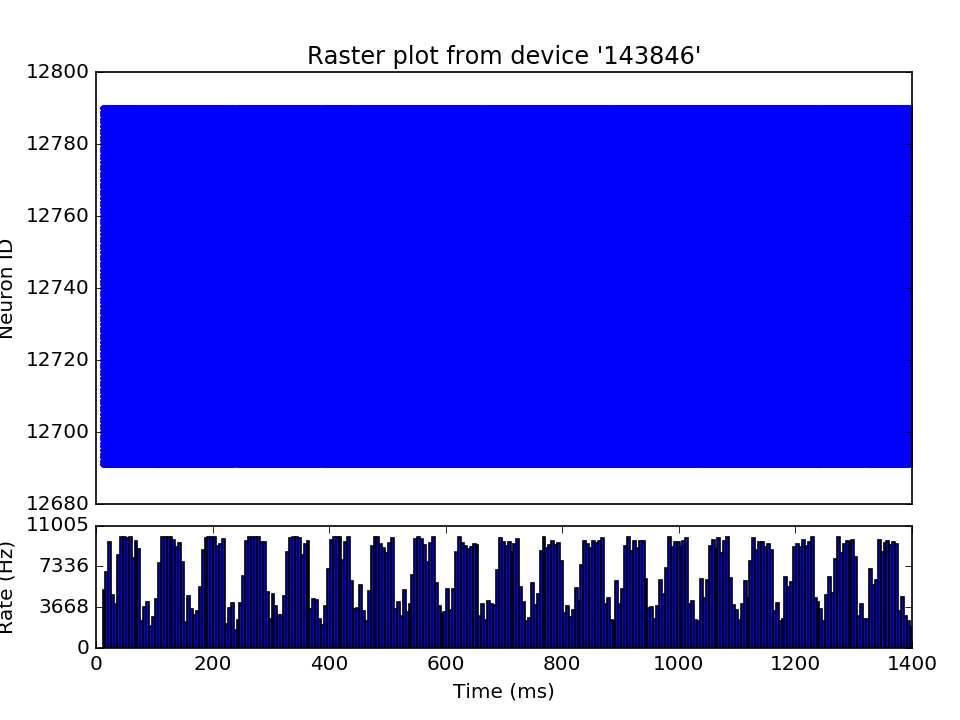
\includegraphics[width=0.5\linewidth]{spikes_rn[dr]}
	\caption{Спайковая активность в ядрах шва.}
	\label{fig:spikes_rn}
\end{figure}

\begin{figure}
	\centering
	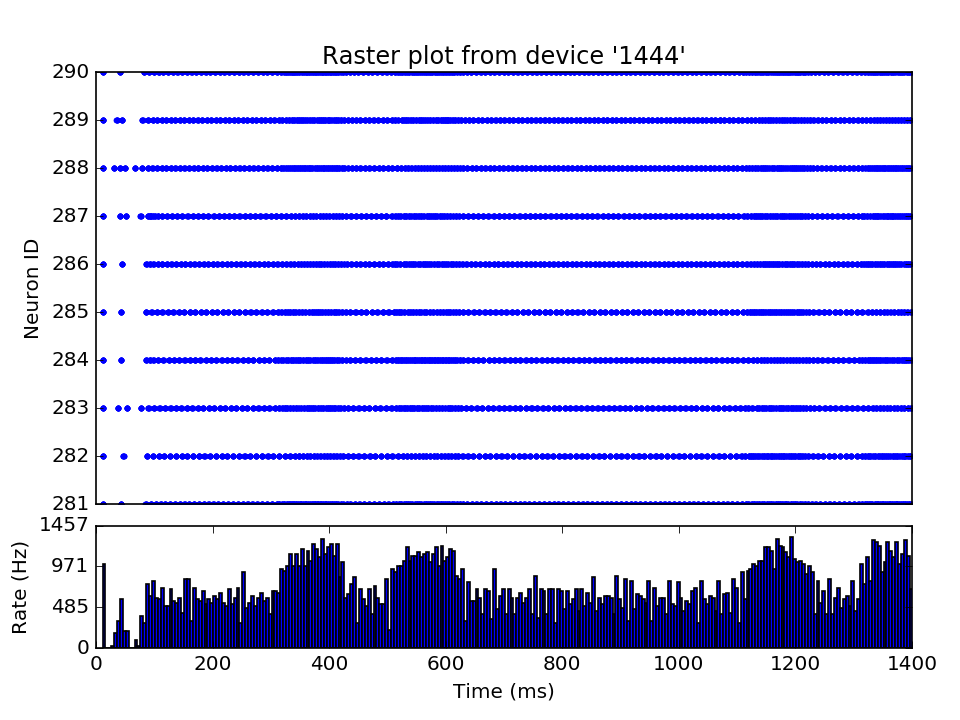
\includegraphics[width=0.5\linewidth]{spikes_snc[da]}
	\caption{Спайковая активность в чёрной субстанции pars compacta.}
	\label{fig:spikes_snc}
\end{figure}

На рис. ~\ref{fig:spikes_rn} активность в ядрах шва, главном центре серотонина, не утихает ни в один момент времени, кроме промежутков с приостановленными генераторами (эмоция стыд), поскольку эта область мозга нагружена проекциями из множества областей. На ядра шва проецируется норадреналин, но отслеживание этого при такой активности затруднено: количество проекций на ядра шва значительно больше, чем на другие области, задействованные в симуляции. Дофаминовый центр, чёрная субстанция pars compacta, максимально активен в положенные ему моменты активации дофамина: на 400 мс (страх), 600 мс (ярость) 1200 мс (радость), 1400 мс (интерес).

\begin{figure}
	\centering
	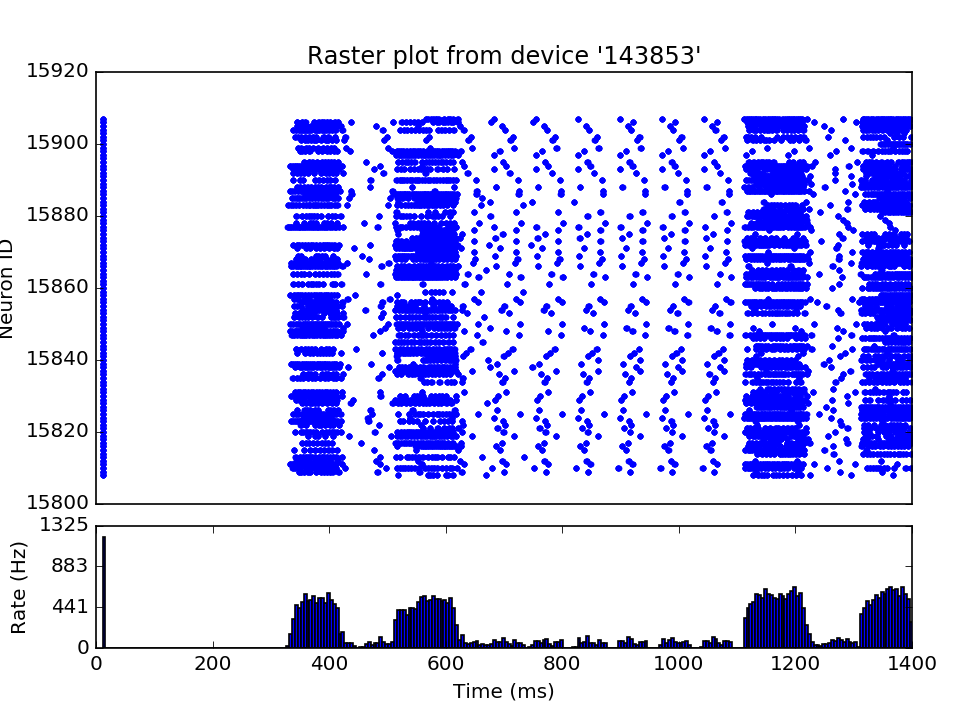
\includegraphics[width=0.5\linewidth]{spikes_vta[da0]}
	\caption{Спайковая активность в вентральной области покрышки.}
	\label{fig:spikes_vta}
\end{figure}

Вентральная область покрышки является интерфейсом взаимодействия всех трёх нейромедиаторов, влияет на их работу, а нейромедиаторы влияют на неё. На рис. ~\ref{fig:spikes_vta} показано, что максимальное влияние оказывает норадреналин (400 мс, 600 мс, 1200 мс, 1400 мс), поскольку проецируется одновременно из всех норадреналиновых центров.

\begin{figure}
	\centering
	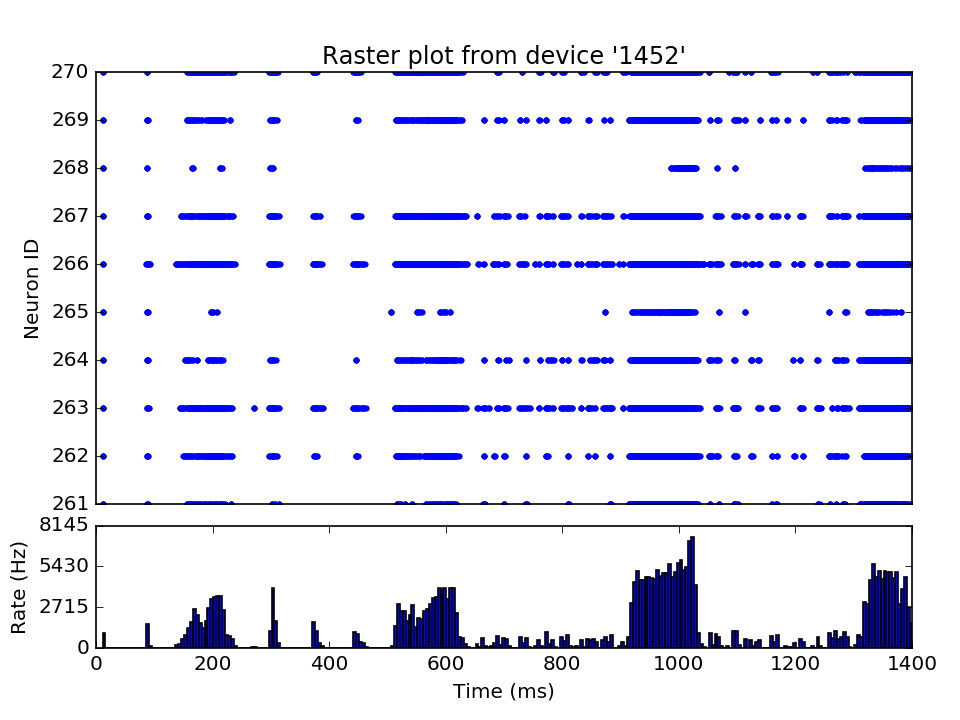
\includegraphics[width=0.5\linewidth]{spikes_striatum[tan]}
	\caption{Спайковая активность в стриатуме (тонические нейроны).}
	\label{fig:spikes_striatum}
\end{figure}

\begin{figure}
	\centering
	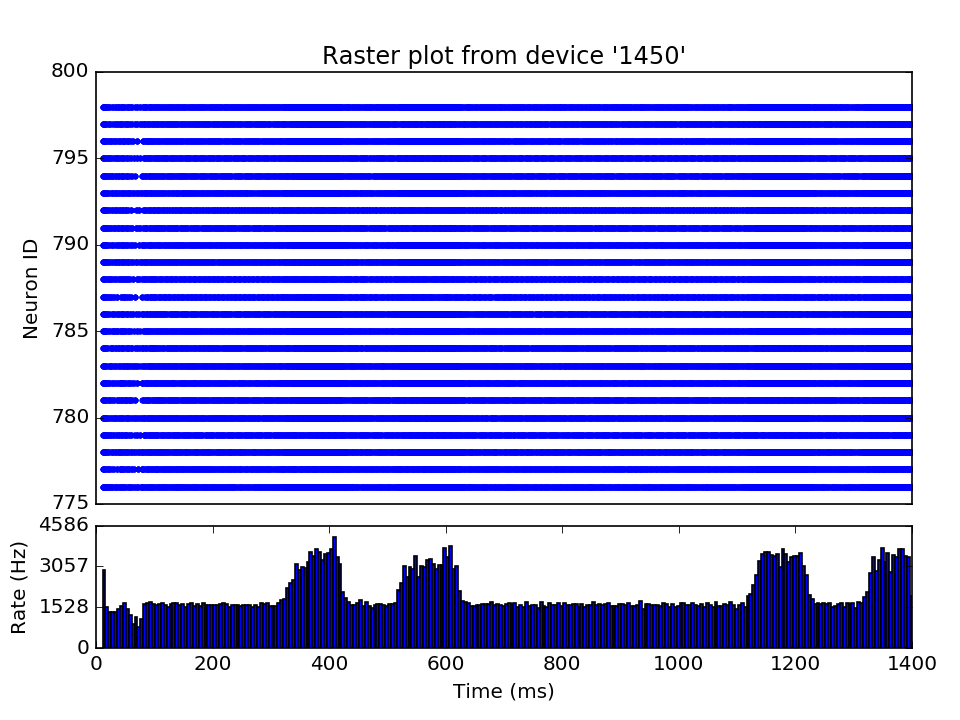
\includegraphics[width=0.5\linewidth]{spikes_striatum[d1]}
	\caption{Спайковая активность в стриатуме (допаминергические нейроны).}
	\label{fig:spikes_striatumх[d1]}
\end{figure}


На рис. ~\ref{fig:spikes_striatum} в тонических нейронах стриатума активность максимальна при высоких уровнях концентрации норадреналина: 200 мс (горе), 600 мс (ярость), 1000 мс (удивление) и 1400 мс (интерес), но также есть спайки при остальных эмоциях, кроме эмоции стыда. Один из дофаминовых центров, чёрная субстанция pars compacta, оказывает непосредственное возбуждающее воздействие на стриатум. Суммарно это влияние более слабое, чем воздействие на стриатум сразу всех норадреналиновых центров. Серотонин оказывает на стриатум ингибирующее воздействие на 700 мс (отвращение), но оно не перекрывает возбуждающее влияние норадреналина на 900 мс (удивление). Наибольшая же часть стриатума активируется сильнее всего дофамином, рис. ~\ref{fig:spikes_striatum}: на 400 мс (страх), 600 мс (ярость), 1200 мс (радость), 1400 мс (интерес).


Спайковая активность в таламусе .................., рис. ~\ref{fig:spikes_thalamus}.
Добавлю гипоталамус. Зря без него.

\begin{figure}
	\centering
	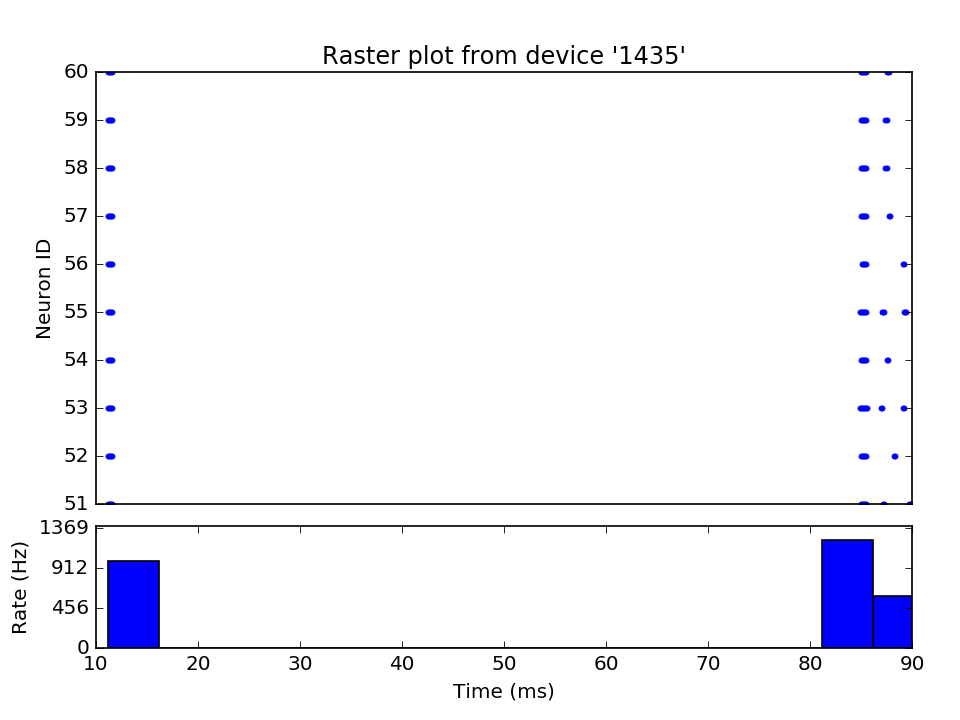
\includegraphics[width=0.5\linewidth]{spikes_thalamus}
	\caption{Спайковая активность в таламусе.}
	\label{fig:spikes_thalamus}
\end{figure}

Моторная и префронтальная кора взаимодействуют со всеми тремя нейромедиаторами, являются связующими звеньями, индикаторами, участвуют в замкнутых циклах (например, префронтальная кора с ядрами шва, моторная кора с голубоватым пятном). На рис. ~\ref{fig:spikes_motor} моторная кора активна на протяжение всей симуляции, сильнее всего завязана на норадреналин и активно испытывает его возбуждающее воздействие на 200 мс, 600 мс, 1000 мс, 1400 мс. Наименьшее количество и наименьшая сила спайков в моторной коре на 700--800 мс (отвращение), что неслучайно: повышенная концентрация серотонина оказывает ингибирующее воздействие, блокируя часть возбуждающих сигналов. Наглядно видна борьба этого воздействия с норадреналиновым возбуждающим на 1000 мс (удивление): спайки более редкие и слабые, чем на 200 мс (горе), когда серотонин не вмешивается в работу норадреналина.


На рис. ~\ref{fig:spikes_prefrontal} спайки на префронтальной коре.....................

\begin{figure}
	\centering
	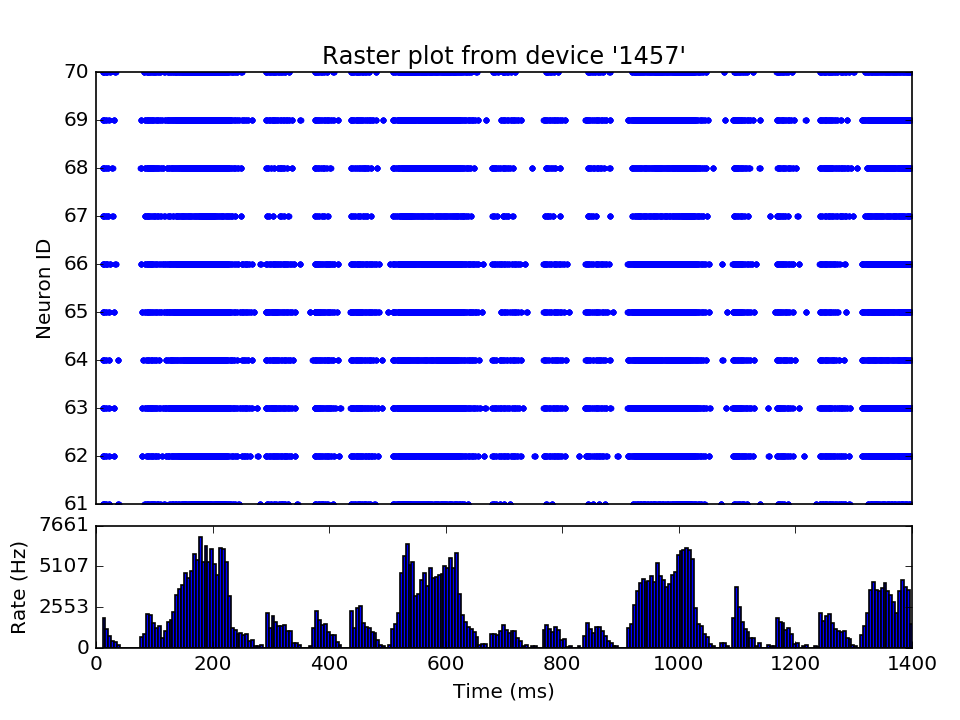
\includegraphics[width=0.5\linewidth]{spikes_motor[glu1]}
	\caption{Спайковая активность в моторной коре.}
	\label{fig:spikes_motor}
\end{figure}

\begin{figure}
	\centering
	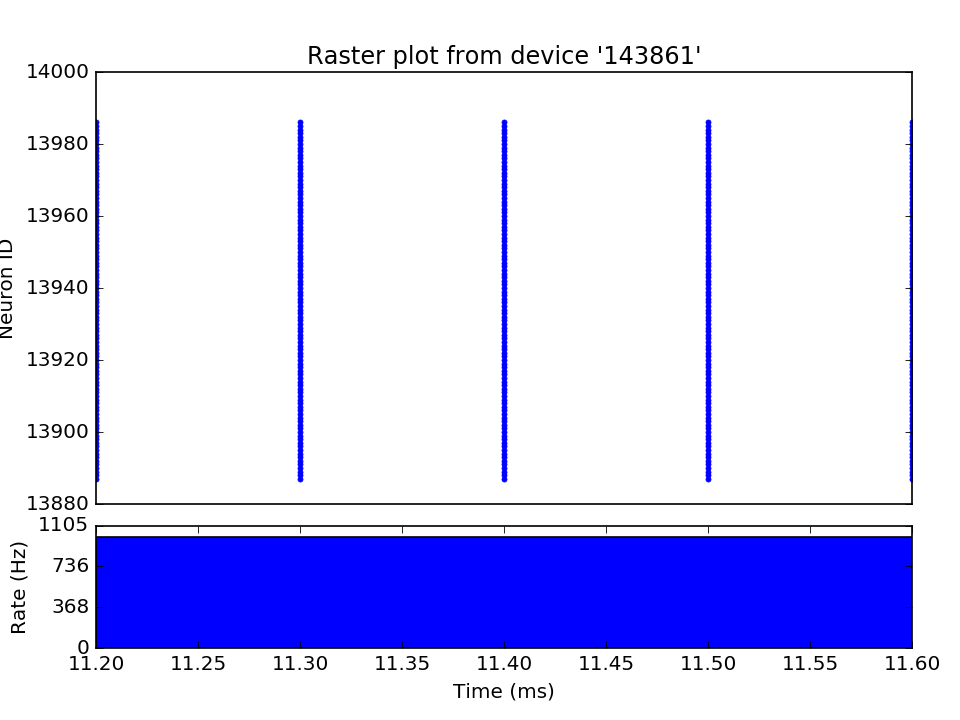
\includegraphics[width=0.5\linewidth]{spikes_prefrontal}
	\caption{Спайковая активность в префронтальной коре.}
	\label{fig:spikes_prefrontal}
\end{figure}




